\documentclass[titlepage,a4paper,twoside]{article}
\usepackage{prettyref}
\usepackage{hyperref}
\usepackage{graphicx}
\usepackage{caption}
\usepackage{subcaption}
\usepackage{xspace}
\usepackage[left=3cm,right=2cm,top=3cm,bottom=5cm,includeheadfoot]{geometry}

\title{MarVis-Graph User Manual}
\author{Manuel Landesfeind}


\newcommand{\mg}{MarVis--Graph\xspace}
\newrefformat{fig}{Figure \ref{#1} ``\nameref{#1}''}
\newrefformat{tab}{Table \ref{#1} ``\nameref{#1}''}
\newrefformat{sec}{Section \ref{#1} ``\nameref{#1}''}
\newrefformat{ssec}{Subsection \ref{#1} ``\nameref{#1}''}
\newrefformat{sssec}{Subsection \ref{#1} ``\nameref{#1}''}
\newcommand{\pref}[1]{\prettyref{#1}}


\begin{document}
\maketitle

\section{Introduction}


\section{Installation}

A \mg installer is available as supplemental material to our paper
\cite{landesfeind2013marvisgraph} or may be downloaded at:
\url{http://marvis.gobics.de}
To install \mg, follow the instructions of the installer. After successfull
installation, \mg can be started via your applications menu.

\subsection{Prerequirements} For the installer and for \mg itself, the Java
Runtime Environment v1.7 (JRE7) or higher is required. JRE7 can be downloaded
(if it is not already installed) free of charge at \url{http://www.java.com}

\mg has been developed on an 64-bit system with Ubuntu Linux 12.10 ``Quantal Quetzal''
\footnote{\url{http://www.ubuntu.com}} using the Netbeans IDE 7
\footnote{\url{https://netbeans.org/}}. Additionally, \mg has been used under
Windows 7\footnote{\url{http://windows.microsoft.com}}. It has \textbf{not}
been tested under Mac OSX and is therefore not supported on Mac. 

\section{User Interface}
\begin{figure}
	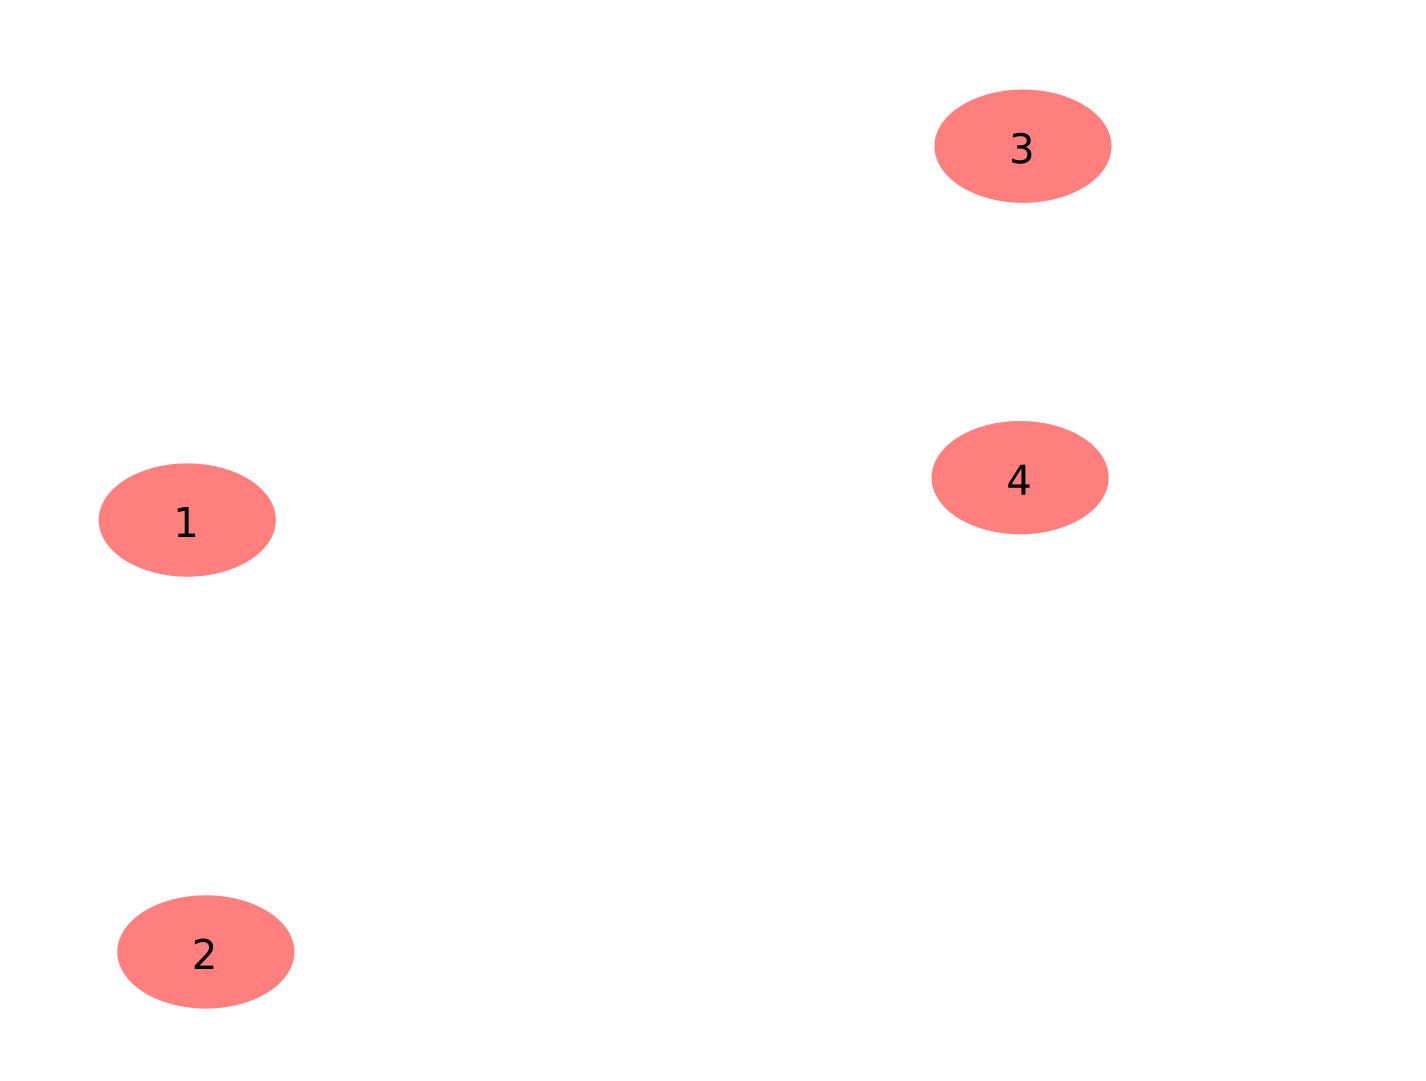
\includegraphics[width=\textwidth]{images/main.pdf}
	\caption[\mg main window]{\mg main window: 1) list of the main network and
		sub--networks sorted according to the selected scoring method. 2)
		Basic information about the contents of the selected network. 3) Setup
		the visualization of the network. 4) Visualization of the network.
		\label{fig:main}}
\end{figure}
The \mg main window, shown in \pref{fig:main}, displays informations in
different areas.

\subsection{Network/Sub--Network list}

On the left side a tree structure displays the different networks calculated.
The root of the tree, i.e. the upper node, is the main network where all
database and experimental data has been integrated. The networks below are
calculated sub--network. When sub--networks are calculated, this tree changes:
first the old sub--networks are irrevocably removed and afterwards the newly
calculated networks are added.

\paragraph{Sorting} The sub--networks can be sorted according to different
scoring methods (see \pref{sssec:scoring}). On top of the sub--network tree a
box is displayed providing accession to the different scoring methods. On
selection of a different method the scores are recalculated and the tree view
is updated.

\section{Using \mg}

\subsection{Building a new network from the database sources}

Before experimental data can be imported into \mg, a metabolic network model
has to be created. \mg currently supports the KEGG and BioCyc database
collections.

While the BioCyc database collection contains more organism--specific networks
from which some are manually curated, the usage of KEGG is preferred as the
download can be done fully automatically.

\begin{figure}
	\begin{subfigure}[b]{0.45\textwidth}
		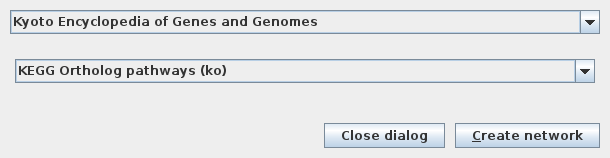
\includegraphics[width=\textwidth]{images/create_network_kegg.png}
		\caption{Create network from KEGG\label{fig:newnetwork_kegg}}
	\end{subfigure}
	\begin{subfigure}[b]{0.45\textwidth}
		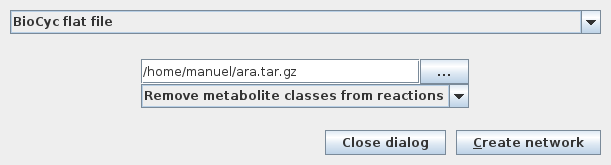
\includegraphics[width=\textwidth]{images/create_network_biocyc.png}
		\caption{Create network from Biocyc\label{fig:newnetwork_biocyc}}
	\end{subfigure}

	\caption[Create new network]{Create a new metabolic network model.
		Depending on the selection between KEGG and Biocyc the options of the
	dialog change. The options are described in \pref{ssec:newnetwork}
	\label{fig:newnetwork}}
\end{figure}

\paragraph{KEGG: Kyoto Encyclopedia of Genes and Genomes}
\cite{kanehisa2010kegg,kanehisa2000kegg} Creating a new metabolic network
model from the KEGG database is done via the KEGG REST
API\footnote{\url{http://www.kegg.jp/kegg/rest}}. 

When KEGG is selected as source in the upper drop--down menu (see
\pref{fig:newnetwork_kegg}), a request is
send to the KEGG webservice to fetch a full list of organisms available.
Afterwards, the organism under research can be selected in the lower
drop--down menu. If no such organism is available the ``KEGG Ortholog Pathways
(KO)'' may be used. This metabolic network contains all reactions in KEGG
(reference network).

Please note that the transmission of data from the KEGG webservice is slow and
the creation may take a while. However, a progressbar will
pop up and display the progress.

\paragraph{BioCyc database collection} \cite{caspi2008metacyc,
caspi2010metacyc,caspi2012metacyc} To create a metabolic network model from
a BioCyc database, the first step is the manual download of the database
because of the license requirements from BioCyc.
After a request for the ``Data File License''
\footnote{\url{http://biocyc.org/download.shtml}} one will receive an email
containing a link to the download page. Here, all individual databases are
listed and the required database can be downloaded as ``tarball'' (file
extension: ``.tar.gz'' or ``.tgz'').
In the \mg dialog for network creation using the BioCyc flat files (see
\pref{fig:newnetwork_biocyc}), the priviously downloaded file has to be selected. 

The import of BioCyc databases requires a specific option determining the
handling of metabolite classes in reactions:
\begin{description}
	\item[Remove metabolite classes from reactions]
		All classes are removed from the reactions resulting in a more sparse
		network. Therefore, connections between reactions may be missed.
	\item[Use metabolite classes as metabolites]
		Each class is assumed to be a metabolite and used stricly. Unfortunately, the classes have no
		monoisotopic mass and annotating them with experimental evidence is hard.
	\item[Substitute classes with metabolites]
		Each class is substituted by the metabolites it represents. This
		results in reactions with a lot of substrates and products.
	\item[Build reactions for each variant]
		For each reaction with class as reactant, all possible variants of the
		reaction are added as single reaction to the network.
		Therefore, metabolites may be associated with a lot of reaction which
		may later interfere with the hub--metabolite threshold (see
		\pref{ssec:calculate}).
\end{description}
Every option has its advantages and disadvantages and it depends on the
hypothesis to be investigated which representation of classes may be the best.
If in doubt, the proposed strategy is the removal of all metabolite clases
form the reactions.

\subsection{Saving and loading a metabolic network}\label{ssec:saveload}

Metabolic network models can be stored and loaded from \mg using a simple XML
file format. To reduce the required space on the harddisk, the XML may be
compressed utilizing the Lembel--Ziv--77 algorithm (gzip).

After creation of a metabolic network it can be saved to harddisk
via the menu ``File'' $\rightarrow$ ``Save network'' (shortkey Crtl + S). 
After selecting a destination and filename, \mg write all data from the
network into that file. 

Similarily, a network can be (re-)loaded into \mg via the menu ``File''
$\rightarrow$ ``Load network'' (shortkey Crtl + L). After selecting a valid
\mg network file the network is imported and set as root network in the
network tree. Hereby, a previously loaded or created network will be removed
without notification.

\subsection{Importing experimental data}

When a metabolic network model is loaded or created in \mg, experimental
data can be added. \mg loads them from tabular data files. Currently, the
following file formats are supported:
\begin{description}
	\item[Comma--Separated--Values (*.csv)\footnote{\url{http://en.wikipedia.org/wiki/Comma-separated_values}}]
		This text file format is the simplest. On import, several additional
		parameters need to be given, e.g. the cell separator and quote
		character.
	\item[Microsoft Excel (*.xls, *.xls)\footnote{\url{http://office.microsoft.com}}]
		\mg can directly import data from the Excel spreadsheet file format.
		On import, the sheet to be imported needs to be specified.
\end{description}

\subsubsection{Metabolite Marker}

\subsubsection{Transcript Marker}

\subsection{Calculating sub--networks}\label{ssec:calculate}

\subsubsection{Perform a random permutation test}

\subsection{Visualizing and inspecting networks}

\subsubsection{Scoring and ranking} \ref{sssec:scoring}

\subsubsection{Chancing the layout}

\section{Contact}
\mg has been developed at the Department for Bioinformatics at the
Georg--August--University in G\"ottingen (Germany).
If you have question or suggestions regarding the software, please write to
\href{mailto:marvis@gobics.de}{marvis@gobics.de}.

\subsection{License}
\mg is released under the terms of the GNU General Public License
v3\footnote{\url{http://www.gnu.org/licenses/gpl-3.0.txt}}> 

\begin{quote}\mg is free software: you can redistribute it and/or modify
    it under the terms of the GNU General Public License as published by
    the Free Software Foundation, either version 3 of the License, or
    (at your option) any later version.

    This program is distributed in the hope that it will be useful,
    but WITHOUT ANY WARRANTY; without even the implied warranty of
    MERCHANTABILITY or FITNESS FOR A PARTICULAR PURPOSE.  See the
    GNU General Public License for more details.

    You should have received a copy of the GNU General Public License
	along with this program.  If not, see \url{http://www.gnu.org/licenses}.
\end{quote}

Usage of \mg is free of charge in academic research. Commercial users please
contact \href{mailto:marvis@gobics.de}{marvis@gobics.de} for license
information.

\subsection{Cite}

If you use \mg in your research, please cite:
\cite{landesfeind2013marvisgraph}


\bibliographystyle{plain}
\bibliography{../../promotion/Library}

\end{document}

